\documentclass{report}
\usepackage[margin=2cm, bottom=1.5cm]{geometry}
\usepackage{type1cm}
\usepackage{amssymb}
\usepackage[fleqn]{amsmath}
\usepackage{tikz}
\usepackage{multicol}
\usepackage{makecell}
\usepackage{tabularx}
\usepackage[shortlabels]{enumitem}
\setlength{\columnsep}{1pt}
\setlist[enumerate]{nosep}

\makeatletter
\newenvironment{myalign*}{\ifvmode\else\hfil\null\linebreak\fi
  \hspace*{-\leftmargin}\minipage\textwidth
  \setlength{\abovedisplayskip}{0pt}%
  \setlength{\abovedisplayshortskip}{\abovedisplayskip}%
  \start@align\@ne\st@rredtrue\m@ne}%
{\endalign\endminipage\linebreak}

\usepackage{xeCJK}
\setCJKmainfont{Noto Sans TC}

\begin{document}
\title{%
  \fontsize{40}{60}\selectfont
  AMM  \\ % 
  \vspace*{2cm}%
  \fontsize{24}{30}\selectfont
  設計文件
}

\author{
  \fontsize{18}{28}\selectfont
  \begin{tabularx}{0.9\textwidth}{
    |p{\dimexpr.25\linewidth-6\tabcolsep-2\arrayrulewidth}%
    |p{\dimexpr.75\linewidth-6\tabcolsep-2\arrayrulewidth}|%
  }
    \hline
    \centering 專案名稱 & AMM 開發輔助工具 \\
    \hline
    \centering 撰寫日期 & 2022 / 11 / 21 \\
    \hline
    \centering 發展者 & 簡蔚驊 \! 鄧暐宣 \! 余威霆 \! 林佳何 \! 唐劭賢 \\
    \hline
  \end{tabularx}
}
\date{}
\usetikzlibrary{automata, positioning, arrows}
\maketitle
\tikzset{every state, accepting/.style={double distance=2pt}}

\fontsize{12}{18}\selectfont

\section*{1. 系統模型與架構(System Model/System Architecture)}

\begin{obeylines}
\parindent=0pt
描述系統之架構。可用C4 model的Container diagram + Component diagram、UML之Component diagram或單純的Block diagram (方塊圖)表達此系統包含的模組,以及與模組之間的關係。
架構圖應與SRS一致,但可特別強調介面(Interface)與實際佈署之環境。
放C4所有的圖片
鄧
\end{obeylines}

\section*{2. 介面需求與設計(Interface Requirement and Design)}

\begin{obeylines}
\parindent=0pt
根據架構圖,描述模組間的介面資訊,包含介面名稱、介面提供者、介面使用者、連結方式、輸入資料、輸出資料與介面描述等。
APIIIIIIIIIIIIIIIIIIIIIIIIIIIIIIIIIIIIIIIIIIIIIIIIIIIIII
簡
\end{obeylines}

% \newcolumntype{R}{>{\raggedleft}X}
\newcolumntype{R}{X}
\newcolumntype{T}{>{\hsize=\dimexpr2\hsize+2\tabcolsep+\arrayrulewidth\relax}X}
\newcolumntype{F}{>{\hsize=\dimexpr4\hsize+4\tabcolsep+\arrayrulewidth\relax}X}

\begin{tabularx}{\textwidth}{|l|R|R|R|}
  \hline
  介面編號 & 介面名稱 & 介面提供者 & 介面使用者 \\ \hline
  [介面編號] & [XXX] & [介面提供者] & [介面使用者] \\ \hline
  連結方式 & \multicolumn{2}{|c|}{輸入資料} & 輸出資料 \\ \hline
  [連結方式] & \multicolumn{2}{|T|}{[輸入資料]} & [輸出資料] \\ \hline
  \multicolumn{4}{|c|}{對應介面之要求} \\ \hline
  \multicolumn{4}{|F|}{[對應介面之要求]} \\ \hline
\end{tabularx}

\subsection*{2.1 會員子系統}

\subsubsection*{2.1.1 外部介面}

\begin{tabularx}{\textwidth}{|l|R|R|R|}
  \hline
  介面編號 & 介面名稱 & 介面提供者 & 介面使用者 \\ \hline
  AMM-EI-01 & 登入帳號 & Account Management Module & User \\ \hline
  連結方式 & \multicolumn{2}{|c|}{輸入資料} & 輸出資料 \\ \hline
   & \multicolumn{2}{|T|}{email, password} & 登入成功後跳轉頁面 \\ \hline
  \multicolumn{4}{|c|}{對應介面之要求} \\ \hline
  \multicolumn{4}{|F|}{
    接收email及password,交由firebase驗證。驗證成功後,回傳token到前端。} \\ \hline
\end{tabularx}

\subsubsection*{}
\begin{tabularx}{\textwidth}{|l|R|R|R|}
  \hline
  介面編號 & 介面名稱 & 介面提供者 & 介面使用者 \\ \hline
  AMM-EI-02 & 註冊帳號 & Account Management Module & Any \\ \hline
  連結方式 & \multicolumn{2}{|c|}{輸入資料} & 輸出資料 \\ \hline
   & \multicolumn{2}{|T|}{email, password} & 註冊成功後跳轉頁面 \\ \hline
  \multicolumn{4}{|c|}{對應介面之要求} \\ \hline
  \multicolumn{4}{|F|}{
    接收email及password,交由firebase註冊。} \\ \hline
\end{tabularx}

\subsubsection*{}
\begin{tabularx}{\textwidth}{|l|R|R|R|}
  \hline
  介面編號 & 介面名稱 & 介面提供者 & 介面使用者 \\ \hline
  AMM-EI-03 & 忘記密碼 & Account Management Module & User \\ \hline
  連結方式 & \multicolumn{2}{|c|}{輸入資料} & 輸出資料 \\ \hline
   & \multicolumn{2}{|T|}{email} & 驗證完後跳回登入頁 \\ \hline
  \multicolumn{4}{|c|}{對應介面之要求} \\ \hline
  \multicolumn{4}{|F|}{
    接收email,交由firebase驗證,並由firebase寄送驗證信到使用者上。} \\ \hline
\end{tabularx}

\subsubsection*{}
\begin{tabularx}{\textwidth}{|l|R|R|R|}
  \hline
  介面編號 & 介面名稱 & 介面提供者 & 介面使用者 \\ \hline
  AMM-EI-04 & 修改個人資料 & Account Management Module & User \\ \hline
  連結方式 & \multicolumn{2}{|c|}{輸入資料} & 輸出資料 \\ \hline
   & \multicolumn{2}{|T|}{avatar url, nickname, bio} & 顯示新的個人資料 \\ \hline
  \multicolumn{4}{|c|}{對應介面之要求} \\ \hline
  \multicolumn{4}{|F|}{
    接收收avatar url、nickname、bio,將資料交給firebase儲存。} \\ \hline
\end{tabularx}

\subsubsection*{}
\begin{tabularx}{\textwidth}{|l|R|R|R|}
  \hline
  介面編號 & 介面名稱 & 介面提供者 & 介面使用者 \\ \hline
  AMM-EI-05 & 修改密碼 & Account Management Module & User \\ \hline
  連結方式 & \multicolumn{2}{|c|}{輸入資料} & 輸出資料 \\ \hline
   & \multicolumn{2}{|T|}{old password, new password} & 跳到登入畫面 \\ \hline
  \multicolumn{4}{|c|}{對應介面之要求} \\ \hline
  \multicolumn{4}{|F|}{
    接收old password、new password,old password與firebase驗證過後,將new password交給firebase做更新。} \\ \hline
\end{tabularx}

\subsubsection*{}
\begin{tabularx}{\textwidth}{|l|R|R|R|}
  \hline
  介面編號 & 介面名稱 & 介面提供者 & 介面使用者 \\ \hline
  AMM-EI-06 & Google 日曆授權 & Account Management Module & User \\ \hline
  連結方式 & \multicolumn{2}{|c|}{輸入資料} & 輸出資料 \\ \hline
   & \multicolumn{2}{|T|}{} &  \\ \hline
  \multicolumn{4}{|c|}{對應介面之要求} \\ \hline
  \multicolumn{4}{|F|}{
    透過Google日曆 API 管理授權} \\ \hline
\end{tabularx}

\subsubsection*{}
\begin{tabularx}{\textwidth}{|l|R|R|R|}
  \hline
  介面編號 & 介面名稱 & 介面提供者 & 介面使用者 \\ \hline
  AMM-EI-07 & 取得通知 & Account Management Module & User \\ \hline
  連結方式 & \multicolumn{2}{|c|}{輸入資料} & 輸出資料 \\ \hline
   & \multicolumn{2}{|T|}{} &  \\ \hline
  \multicolumn{4}{|c|}{對應介面之要求} \\ \hline
  \multicolumn{4}{|F|}{
    系統上顯示傳給使用者的通知} \\ \hline
\end{tabularx}

\subsubsection*{2.1.2 內部介面}

\subsubsection*{}
\begin{tabularx}{\textwidth}{|l|R|R|R|}
  \hline
  介面編號 & 介面名稱 & 介面提供者 & 介面使用者 \\ \hline
  AMM-II-01 & /signin & Account Management Module & User \\ \hline
  連結方式 & \multicolumn{2}{|c|}{輸入資料} & 輸出資料 \\ \hline
 POST & \multicolumn{2}{|T|}{
    \makecell[l]{
      \{ \\
        "email": "Email (string)", \\
        "password": "Password (string)" \\
      \}      
    }
   } & 
   \makecell[X]{
    \{ \\
      "status": "Status (string, 200)", \\
      "JWT": "JWT token (string)" \\
    \}
    }
   \\ \hline
  \multicolumn{4}{|c|}{對應介面之要求} \\ \hline
  \multicolumn{4}{|F|}{
    將登入資訊傳給firebase進行資料驗證,接收回傳結果} \\ \hline
\end{tabularx}

\subsubsection*{}
\begin{tabularx}{\textwidth}{|l|R|R|R|}
  \hline
  介面編號 & 介面名稱 & 介面提供者 & 介面使用者 \\ \hline
  AMM-II-02 & /signup & Account Management Module & User \\ \hline
  連結方式 & \multicolumn{2}{|c|}{輸入資料} & 輸出資料 \\ \hline
 POST & \multicolumn{2}{|T|}{
    \makecell[l]{
      \{ \\
        "email": "Email (string)", \\
        "password": "Password (string)" \\
      \}      
    }
   } & 
   \makecell[X]{
    \{ \\
      "status": "Status (string, 200)", \\
      "JWT": "JWT token (string)" \\
    \}
    }
   \\ \hline
  \multicolumn{4}{|c|}{對應介面之要求} \\ \hline
  \multicolumn{4}{|F|}{
    將註冊資訊傳給firebase,驗證後加入資料庫} \\ \hline
\end{tabularx}

\subsubsection*{}
\begin{tabularx}{\textwidth}{|l|R|R|R|}
  \hline
  介面編號 & 介面名稱 & 介面提供者 & 介面使用者 \\ \hline
  AMM-II-03 & /forget & Account Management Module & User \\ \hline
  連結方式 & \multicolumn{2}{|c|}{輸入資料} & 輸出資料 \\ \hline
 POST & \multicolumn{2}{|T|}{
    \makecell[l]{
      \{ \\
        "email": "Email (string)", \\
      \}      
    }
   } & 
   \makecell[X]{
    \{ \\
      "status": "Status (string, 200)",
    \}
    }
   \\ \hline
  \multicolumn{4}{|c|}{對應介面之要求} \\ \hline
  \multicolumn{4}{|F|}{
    傳送email,交給firebase寄信重設密碼} \\ \hline
\end{tabularx}

\subsubsection*{}
\begin{tabularx}{\textwidth}{|l|R|R|R|}
  \hline
  介面編號 & 介面名稱 & 介面提供者 & 介面使用者 \\ \hline
  AMM-II-04 & /person & Account Management Module & User \\ \hline
  連結方式 & \multicolumn{2}{|c|}{輸入資料} & 輸出資料 \\ \hline
 PUT & \multicolumn{2}{|T|}{
    \makecell[l]{
      \{ \\
        "JWT": "JWT token (string, cookie)", \\
        "avatar": "Avatar (base64)", \\
        "nickname": "Nickname (string)", \\
        "bio": "bio (string)" \\
      \}      
    }
   } & 
   \makecell[X]{
    \{ \\
      "status": "Status (string, 200)",
    \}
    }
   \\ \hline
  \multicolumn{4}{|c|}{對應介面之要求} \\ \hline
  \multicolumn{4}{|F|}{
    將個人資訊傳給firebase,根據avatar找到帳戶進行儲存,回傳狀態} \\ \hline
\end{tabularx}

\subsubsection*{}
\begin{tabularx}{\textwidth}{|l|R|R|R|}
  \hline
  介面編號 & 介面名稱 & 介面提供者 & 介面使用者 \\ \hline
  AMM-II-05 & /person & Account Management Module & User \\ \hline
  連結方式 & \multicolumn{2}{|c|}{輸入資料} & 輸出資料 \\ \hline
 GET & \multicolumn{2}{|T|}{
    \makecell[l]{
      \{ \\
        "JWT": "JWT token (string, cookie)", \\
        "email": "Email (string)", \\
      \}      
    }
   } & 
   \makecell[X]{
    \{ \\
      "status": "Status (string, 200)",
    \}
    }
   \\ \hline
  \multicolumn{4}{|c|}{對應介面之要求} \\ \hline
  \multicolumn{4}{|F|}{
    獲取資料} \\ \hline
\end{tabularx}

\subsubsection*{}
\begin{tabularx}{\textwidth}{|l|R|R|R|}
  \hline
  介面編號 & 介面名稱 & 介面提供者 & 介面使用者 \\ \hline
  AMM-II-06 & /person/reset & Account Management Module & User \\ \hline
  連結方式 & \multicolumn{2}{|c|}{輸入資料} & 輸出資料 \\ \hline
 POST & \multicolumn{2}{|T|}{
    \makecell[l]{
      \{ \\
       "JWT": "JWT token (string, cookie)", \\
        "oldPassword": "Password (string)", \\
        "newPassword": "Password (string)", \\
      \}      
    }
   } & 
   \makecell[X]{
    \{ \\
      "status": "Status (string, 200)",
    \}
    }
   \\ \hline
  \multicolumn{4}{|c|}{對應介面之要求} \\ \hline
  \multicolumn{4}{|F|}{
    改密碼} \\ \hline
\end{tabularx}

\subsubsection*{}
\begin{tabularx}{\textwidth}{|l|R|R|R|}
  \hline
  介面編號 & 介面名稱 & 介面提供者 & 介面使用者 \\ \hline
  AMM-II-07 & /person/calendar & Account Management Module & User \\ \hline
  連結方式 & \multicolumn{2}{|c|}{輸入資料} & 輸出資料 \\ \hline
 POST & \multicolumn{2}{|T|}{
    \makecell[l]{
      \{ \\
        "JWT": "JWT token (string, cookie)", \\
        \}      
    }
   } & 
   \makecell[X]{
    \{ \\
      "status": "Status (string, 200)",
    \}
    }
   \\ \hline
  \multicolumn{4}{|c|}{對應介面之要求} \\ \hline
  \multicolumn{4}{|F|}{
    接收資料後} \\ \hline
\end{tabularx}

\subsubsection*{}
\begin{tabularx}{\textwidth}{|l|R|R|R|}
  \hline
  介面編號 & 介面名稱 & 介面提供者 & 介面使用者 \\ \hline
  AMM-II-08 & /notify & Account Management Module & User \\ \hline
  連結方式 & \multicolumn{2}{|c|}{輸入資料} & 輸出資料 \\ \hline
 GET & \multicolumn{2}{|T|}{
    \makecell[l]{
      \{ \\
        "JWT": "JWT token (string, cookie)", \\
      \}      
    }
   } & 
   \makecell[X]{
    \{ \\
      "status": "Status (string, 200)",
    \}
    }
   \\ \hline
  \multicolumn{4}{|c|}{對應介面之要求} \\ \hline
  \multicolumn{4}{|F|}{
    接收資料後} \\ \hline
\end{tabularx}

\subsection*{2.2 專案管理子系統}

\subsubsection*{2.2.1 外部介面}

\subsubsection*{}
\begin{tabularx}{\textwidth}{|l|R|R|R|}
  \hline
  介面編號 & 介面名稱 & 介面提供者 & 介面使用者 \\ \hline
  PMM-EI-01 & 列出所有專案 & Project Management Module & User \\ \hline
  連結方式 & \multicolumn{2}{|c|}{輸入資料} & 輸出資料 \\ \hline
   & \multicolumn{2}{|T|}{
    \makecell[l]{}
   } & 
   \makecell[X]{
     列出所有專案的資料
    }
   \\ \hline
  \multicolumn{4}{|c|}{對應介面之要求} \\ \hline
  \multicolumn{4}{|F|}{
    } \\ \hline
\end{tabularx}

\subsubsection*{}
\begin{tabularx}{\textwidth}{|l|R|R|R|}
  \hline
  介面編號 & 介面名稱 & 介面提供者 & 介面使用者 \\ \hline
  PMM-EI-02 & 建立新專案 & Project Management Module & User \\ \hline
  連結方式 & \multicolumn{2}{|c|}{輸入資料} & 輸出資料 \\ \hline
   & \multicolumn{2}{|T|}{
    \makecell[l]{
      Project Name, Development Mode
    }
   } & 
   \makecell[X]{
     新增完專案後,跳到專案畫面。
    }
   \\ \hline
  \multicolumn{4}{|c|}{對應介面之要求} \\ \hline
  \multicolumn{4}{|F|}{
    } \\ \hline
\end{tabularx}

\subsubsection*{}
\begin{tabularx}{\textwidth}{|l|R|R|R|}
  \hline
  介面編號 & 介面名稱 & 介面提供者 & 介面使用者 \\ \hline
  PMM-EI-03 & 新建 Readme & Project Management Module & User \\ \hline
  連結方式 & \multicolumn{2}{|c|}{輸入資料} & 輸出資料 \\ \hline
   & \multicolumn{2}{|T|}{
    \makecell[l]{
      % 
    }
   } & 
   \makecell[X]{
     建立 Readme 檔案
    }
   \\ \hline
  \multicolumn{4}{|c|}{對應介面之要求} \\ \hline
  \multicolumn{4}{|F|}{
    } \\ \hline
\end{tabularx}

\subsubsection*{}
\begin{tabularx}{\textwidth}{|l|R|R|R|}
  \hline
  介面編號 & 介面名稱 & 介面提供者 & 介面使用者 \\ \hline
  PMM-EI-04 & 專案設定修改 & Project Management Module & User \\ \hline
  連結方式 & \multicolumn{2}{|c|}{輸入資料} & 輸出資料 \\ \hline
   & \multicolumn{2}{|T|}{
    \makecell[l]{
      Project Name, Development Mode
    }
   } & 
   \makecell[X]{
     修改完專案設定後,跳到專案畫面。
    }
   \\ \hline
  \multicolumn{4}{|c|}{對應介面之要求} \\ \hline
  \multicolumn{4}{|F|}{
    } \\ \hline
\end{tabularx}

\subsubsection*{}
\begin{tabularx}{\textwidth}{|l|R|R|R|}
  \hline
  介面編號 & 介面名稱 & 介面提供者 & 介面使用者 \\ \hline
  PMM-EI-05 & 邀請加入專案 & Project Management Module & User \\ \hline
  連結方式 & \multicolumn{2}{|c|}{輸入資料} & 輸出資料 \\ \hline
   & \multicolumn{2}{|T|}{
    \makecell[l]{
      User Mail
    }
   } & 
   \makecell[X]{
    % 
    }
   \\ \hline
  \multicolumn{4}{|c|}{對應介面之要求} \\ \hline
  \multicolumn{4}{|F|}{
    } \\ \hline
\end{tabularx}

\subsubsection*{}
\begin{tabularx}{\textwidth}{|l|R|R|R|}
  \hline
  介面編號 & 介面名稱 & 介面提供者 & 介面使用者 \\ \hline
  PMM-EI-06 & 移除成員 & Project Management Module & User \\ \hline
  連結方式 & \multicolumn{2}{|c|}{輸入資料} & 輸出資料 \\ \hline
   & \multicolumn{2}{|T|}{
    \makecell[l]{
      User Mail
    }
   } & 
   \makecell[X]{
    %  
    }
   \\ \hline
  \multicolumn{4}{|c|}{對應介面之要求} \\ \hline
  \multicolumn{4}{|F|}{
    } \\ \hline
\end{tabularx}

\subsubsection*{}
\begin{tabularx}{\textwidth}{|l|R|R|R|}
  \hline
  介面編號 & 介面名稱 & 介面提供者 & 介面使用者 \\ \hline
  PMM-EI-07 & 刪除專案 & Project Management Module & User \\ \hline
  連結方式 & \multicolumn{2}{|c|}{輸入資料} & 輸出資料 \\ \hline
   & \multicolumn{2}{|T|}{
    \makecell[l]{
    %  
    }
   } & 
   \makecell[X]{
     刪除完專案,跳回到專案列表。
    }
   \\ \hline
  \multicolumn{4}{|c|}{對應介面之要求} \\ \hline
  \multicolumn{4}{|F|}{
    } \\ \hline
\end{tabularx}

\subsubsection*{2.2.2 內部介面}

\subsubsection*{}
\begin{tabularx}{\textwidth}{|l|R|R|R|}
  \hline
  介面編號 & 介面名稱 & 介面提供者 & 介面使用者 \\ \hline
  PMM-II-01 & /projects & Project Management Module & User \\ \hline
  連結方式 & \multicolumn{2}{|c|}{輸入資料} & 輸出資料 \\ \hline
 GET & \multicolumn{2}{|T|}{
    \makecell[l]{
    %  
    }
   } & 
   \makecell[X]{
     \{
      "projects": "專案列表 (Array<{string, projectid}>)"
     \}
    }
   \\ \hline
  \multicolumn{4}{|c|}{對應介面之要求} \\ \hline
  \multicolumn{4}{|F|}{
  獲取專案列表
  } \\ \hline
\end{tabularx}

\subsubsection*{}
\begin{tabularx}{\textwidth}{|l|R|R|R|}
  \hline
  介面編號 & 介面名稱 & 介面提供者 & 介面使用者 \\ \hline
  PMM-II-02 & /project & Project Management Module & User \\ \hline
  連結方式 & \multicolumn{2}{|c|}{輸入資料} & 輸出資料 \\ \hline
 POST & \multicolumn{2}{|T|}{
    \makecell[l]{
      \{ \\
        "projectname": "project name (string)", \\
        "developmentmode": "development mode (string)", \\
      \}
    }
   } & 
   \makecell[X]{
    %  \{
    %   "projects": "專案列表"
    %  \}
    }
   \\ \hline
  \multicolumn{4}{|c|}{對應介面之要求} \\ \hline
  \multicolumn{4}{|F|}{
  新建專案  
  } \\ \hline
\end{tabularx}

\subsubsection*{}
\begin{tabularx}{\textwidth}{|l|R|R|R|}
  \hline
  介面編號 & 介面名稱 & 介面提供者 & 介面使用者 \\ \hline
  PMM-II-03 & /project/readme & Project Management Module & User \\ \hline
  連結方式 & \multicolumn{2}{|c|}{輸入資料} & 輸出資料 \\ \hline
 POST & \multicolumn{2}{|T|}{
    \makecell[l]{
    %  
    }
   } & 
   \makecell[X]{
    %  \{
    %   "projects": "專案列表"
    %  \}
    }
   \\ \hline
  \multicolumn{4}{|c|}{對應介面之要求} \\ \hline
  \multicolumn{4}{|F|}{
  加 readme  
  } \\ \hline
\end{tabularx}

\subsubsection*{}
\begin{tabularx}{\textwidth}{|l|R|R|R|}
  \hline
  介面編號 & 介面名稱 & 介面提供者 & 介面使用者 \\ \hline
  PMM-II-04 & /project & Project Management Module & User \\ \hline
  連結方式 & \multicolumn{2}{|c|}{輸入資料} & 輸出資料 \\ \hline
 PUT & \multicolumn{2}{|T|}{
    \makecell[l]{
      \{ \\
        "projectname": "project name (string)", \\
        "developmentmode": "development mode (string)", \\
      \}
    }
   } & 
   \makecell[X]{
    %  \{
    %   "projects": "專案列表"
    %  \}
    }
   \\ \hline
  \multicolumn{4}{|c|}{對應介面之要求} \\ \hline
  \multicolumn{4}{|F|}{
  修改專案設定 
  } \\ \hline
\end{tabularx}

\subsubsection*{}
\begin{tabularx}{\textwidth}{|l|R|R|R|}
  \hline
  介面編號 & 介面名稱 & 介面提供者 & 介面使用者 \\ \hline
  PMM-II-05 & /project/member & Project Management Module & User \\ \hline
  連結方式 & \multicolumn{2}{|c|}{輸入資料} & 輸出資料 \\ \hline
 GET & \multicolumn{2}{|T|}{
    \makecell[l]{
      % \{
      %   "projectname": "project name (string)",
      %   "developmentmode": "development mode (string)",
      % \}
    }
   } & 
   \makecell[X]{
    %  \{
    %   "projects": "專案列表"
    %  \}
    }
   \\ \hline
  \multicolumn{4}{|c|}{對應介面之要求} \\ \hline
  \multicolumn{4}{|F|}{
    獲取此專案的成員資料
    } \\ \hline
\end{tabularx}

\subsubsection*{}
\begin{tabularx}{\textwidth}{|l|R|R|R|}
  \hline
  介面編號 & 介面名稱 & 介面提供者 & 介面使用者 \\ \hline
  PMM-II-06 & /project/member & Project Management Module & User \\ \hline
  連結方式 & \multicolumn{2}{|c|}{輸入資料} & 輸出資料 \\ \hline
 POST & \multicolumn{2}{|T|}{
    \makecell[l]{
      \{ \\
        "mail": "User mail (string)", \\
      \}
    }
   } & 
   \makecell[X]{
    %  \{
    %   "projects": "專案列表"
    %  \}
    }
   \\ \hline
  \multicolumn{4}{|c|}{對應介面之要求} \\ \hline
  \multicolumn{4}{|F|}{
  邀請成員 
  } \\ \hline
\end{tabularx}

\subsubsection*{}
\begin{tabularx}{\textwidth}{|l|R|R|R|}
  \hline
  介面編號 & 介面名稱 & 介面提供者 & 介面使用者 \\ \hline
  PMM-II-07 & /project/member & Project Management Module & User \\ \hline
  連結方式 & \multicolumn{2}{|c|}{輸入資料} & 輸出資料 \\ \hline
 DELETE & \multicolumn{2}{|T|}{
    \makecell[l]{
      \{ \\
        "usermail": "User mail (string)", \\
      \}
    }
   } & 
   \makecell[X]{
    %  \{
    %   "projects": "專案列表"
    %  \}
    }
   \\ \hline
  \multicolumn{4}{|c|}{對應介面之要求} \\ \hline
  \multicolumn{4}{|F|}{
  刪除成員 
  } \\ \hline
\end{tabularx}

\subsubsection*{}
\begin{tabularx}{\textwidth}{|l|R|R|R|}
  \hline
  介面編號 & 介面名稱 & 介面提供者 & 介面使用者 \\ \hline
  PMM-II-03 & /project & Project Management Module & User \\ \hline
  連結方式 & \multicolumn{2}{|c|}{輸入資料} & 輸出資料 \\ \hline
 DELETE & \multicolumn{2}{|T|}{
    \makecell[l]{
      % \{
      %   "projectname": "project name (string)",
      %   "developmentmode": "development mode (string)",
      % \}
    }
   } & 
   \makecell[X]{
    %  \{
    %   "projects": "專案列表"
    %  \}
    }
   \\ \hline
  \multicolumn{4}{|c|}{對應介面之要求} \\ \hline
  \multicolumn{4}{|F|}{
   
  移除專案
  } \\ \hline
\end{tabularx}

\subsection*{2.3 Repo管理子系統}

\subsubsection*{2.3.1 外部介面}

\subsubsection*{}
\begin{tabularx}{\textwidth}{|l|R|R|R|}
  \hline
  介面編號 & 介面名稱 & 介面提供者 & 介面使用者 \\ \hline
  RMM-EI-01 & 列出所有REPO & Repo Management Module & User \\ \hline
  連結方式 & \multicolumn{2}{|c|}{輸入資料} & 輸出資料 \\ \hline
   & \multicolumn{2}{|T|}{
    \makecell[l]{}
   } & 
   \makecell[X]{
     列出所有REPO
    }
   \\ \hline
  \multicolumn{4}{|c|}{對應介面之要求} \\ \hline
  \multicolumn{4}{|F|}{
    } \\ \hline
\end{tabularx}

\subsubsection*{}
\begin{tabularx}{\textwidth}{|l|R|R|R|}
  \hline
  介面編號 & 介面名稱 & 介面提供者 & 介面使用者 \\ \hline
  RMM-EI-02 & 新增 REPO & Repo Management Module & User \\ \hline
  連結方式 & \multicolumn{2}{|c|}{輸入資料} & 輸出資料 \\ \hline
   & \multicolumn{2}{|T|}{
    \makecell[l]{
      reponame, repourl
    }
   } & 
   \makecell[X]{
    %  列出所有REPO
    repoid
    }
   \\ \hline
  \multicolumn{4}{|c|}{對應介面之要求} \\ \hline
  \multicolumn{4}{|F|}{
    } \\ \hline
\end{tabularx}

\subsubsection*{}
\begin{tabularx}{\textwidth}{|l|R|R|R|}
  \hline
  介面編號 & 介面名稱 & 介面提供者 & 介面使用者 \\ \hline
  RMM-EI-02 & 刪除 REPO & Repo Management Module & User \\ \hline
  連結方式 & \multicolumn{2}{|c|}{輸入資料} & 輸出資料 \\ \hline
   & \multicolumn{2}{|T|}{
    \makecell[l]{
      repoid
    }
   } & 
   \makecell[X]{
    %  列出所有REPO
    }
   \\ \hline
  \multicolumn{4}{|c|}{對應介面之要求} \\ \hline
  \multicolumn{4}{|F|}{
    } \\ \hline
\end{tabularx}

\subsubsection*{2.3.2 內部介面}

\subsubsection*{}
\begin{tabularx}{\textwidth}{|l|R|R|R|}
  \hline
  介面編號 & 介面名稱 & 介面提供者 & 介面使用者 \\ \hline
  RMM-II-01 & /project/repos & Repo Management Module & User \\ \hline
  連結方式 & \multicolumn{2}{|c|}{輸入資料} & 輸出資料 \\ \hline
  GET & \multicolumn{2}{|T|}{
    \makecell[l]{
      \{ \\
        "projectid": "Project ID (string)" \\
      \}
    }
   } & 
   \makecell[X]{
    \{ \\
      "repos": "REPO列表" \\
    \}
    }
   \\ \hline
  \multicolumn{4}{|c|}{對應介面之要求} \\ \hline
  \multicolumn{4}{|F|}{
    } \\ \hline
\end{tabularx}

\subsubsection*{}
\begin{tabularx}{\textwidth}{|l|R|R|R|}
  \hline
  介面編號 & 介面名稱 & 介面提供者 & 介面使用者 \\ \hline
  RMM-II-02 & /project/repo & Repo Management Module & User \\ \hline
  連結方式 & \multicolumn{2}{|c|}{輸入資料} & 輸出資料 \\ \hline
  POST & \multicolumn{2}{|T|}{
    \makecell[l]{
      \{ \\
        "projectid": "Project ID (string)" \\
        "reponame": "REPO名稱 (string)" \\
        "repourl": "REPO URL (string)" \\
      \}
    }
   } & 
   \makecell[X]{
    \{ \\
      "repoid": "REPO ID (string)" \\
    \}
    }
   \\ \hline
  \multicolumn{4}{|c|}{對應介面之要求} \\ \hline
  \multicolumn{4}{|F|}{
   新增 repo } \\ \hline
\end{tabularx}

\subsubsection*{}
\begin{tabularx}{\textwidth}{|l|R|R|R|}
  \hline
  介面編號 & 介面名稱 & 介面提供者 & 介面使用者 \\ \hline
  RMM-II-03 & /project/repo & Repo Management Module & User \\ \hline
  連結方式 & \multicolumn{2}{|c|}{輸入資料} & 輸出資料 \\ \hline
  PUT & \multicolumn{2}{|T|}{
    \makecell[l]{
      \{ \\
        "projectid": "Project ID (string)" \\
        "repoid": "REPO ID (string)" \\
        "reponame": "REPO名稱 (string)" \\
      \}
    }
   } & 
   \makecell[X]{
    \{ \\
      "repoid": "REPO ID (string)" \\
    \}
    }
   \\ \hline
  \multicolumn{4}{|c|}{對應介面之要求} \\ \hline
  \multicolumn{4}{|F|}{
   修改repo } \\ \hline
\end{tabularx}


\subsubsection*{}
\begin{tabularx}{\textwidth}{|l|R|R|R|}
  \hline
  介面編號 & 介面名稱 & 介面提供者 & 介面使用者 \\ \hline
  RMM-II-02 & /project/repo & Repo Management Module & User \\ \hline
  連結方式 & \multicolumn{2}{|c|}{輸入資料} & 輸出資料 \\ \hline
  DELETE & \multicolumn{2}{|T|}{
    \makecell[l]{
      \{ \\
        "projectid": "Project ID (string)" \\
        "repoid": "Project ID (string)" \\
      \}
    }
   } & 
   \makecell[X]{
    % \{ \\
    %   "repos": "REPO列表" \\
    % \}
    }
   \\ \hline
  \multicolumn{4}{|c|}{對應介面之要求} \\ \hline
  \multicolumn{4}{|F|}{
   刪除repo } \\ \hline
\end{tabularx}

\subsection*{2.4 文件管理子系統}

\subsubsection*{2.4.1 外部介面}

\subsubsection*{}
\begin{tabularx}{\textwidth}{|l|T|X|X|}
  \hline
  介面編號 & 介面名稱 & 介面提供者 & 介面使用者 \\ \hline
  DMM-EI-01 & 列出所有文件 & Doc Management Module & User \\ \hline
  連結方式 & \multicolumn{2}{|c|}{輸入資料} & 輸出資料 \\ \hline
   & \multicolumn{2}{|T|}{
    \makecell[l]{}
   } & 
   \makecell[X]{
    列出所有文件
    }
   \\ \hline
  \multicolumn{4}{|c|}{對應介面之要求} \\ \hline
  \multicolumn{4}{|F|}{
    } \\ \hline
\end{tabularx}

\subsubsection*{}
\begin{tabularx}{\textwidth}{|l|R|R|R|}
  \hline
  介面編號 & 介面名稱 & 介面提供者 & 介面使用者 \\ \hline
  DMM-EI-02 & 新增文件 & Doc Management Module & User \\ \hline
  連結方式 & \multicolumn{2}{|c|}{輸入資料} & 輸出資料 \\ \hline
   & \multicolumn{2}{|T|}{
    \makecell[l]{
      文件類型
    }
   } & 
   \makecell[X]{
    % 列出所有文件
    }
   \\ \hline
  \multicolumn{4}{|c|}{對應介面之要求} \\ \hline
  \multicolumn{4}{|F|}{
    } \\ \hline
\end{tabularx}

\subsubsection*{}
\begin{tabularx}{\textwidth}{|l|R|R|R|}
  \hline
  介面編號 & 介面名稱 & 介面提供者 & 介面使用者 \\ \hline
  DMM-EI-03 & 編輯文件 & Doc Management Module & User \\ \hline
  連結方式 & \multicolumn{2}{|c|}{輸入資料} & 輸出資料 \\ \hline
   & \multicolumn{2}{|T|}{
    \makecell[l]{
      文件類型
    }
   } & 
   \makecell[X]{
    % 列出所有文件
    }
   \\ \hline
  \multicolumn{4}{|c|}{對應介面之要求} \\ \hline
  \multicolumn{4}{|F|}{
    } \\ \hline
\end{tabularx}

\subsubsection*{}
\begin{tabularx}{\textwidth}{|l|R|R|R|}
  \hline
  介面編號 & 介面名稱 & 介面提供者 & 介面使用者 \\ \hline
  DMM-EI-04 & 刪除文件 & Doc Management Module & User \\ \hline
  連結方式 & \multicolumn{2}{|c|}{輸入資料} & 輸出資料 \\ \hline
   & \multicolumn{2}{|T|}{
    \makecell[l]{
      文件類型
    }
   } & 
   \makecell[X]{
    % 列出所有文件
    }
   \\ \hline
  \multicolumn{4}{|c|}{對應介面之要求} \\ \hline
  \multicolumn{4}{|F|}{
    } \\ \hline
\end{tabularx}



\section*{3. 流程設計(Process Design)}

\begin{obeylines}
\parindent=0pt
\begin{enumerate}[label=(\Alph*)]
  \item 會員註冊 \\
  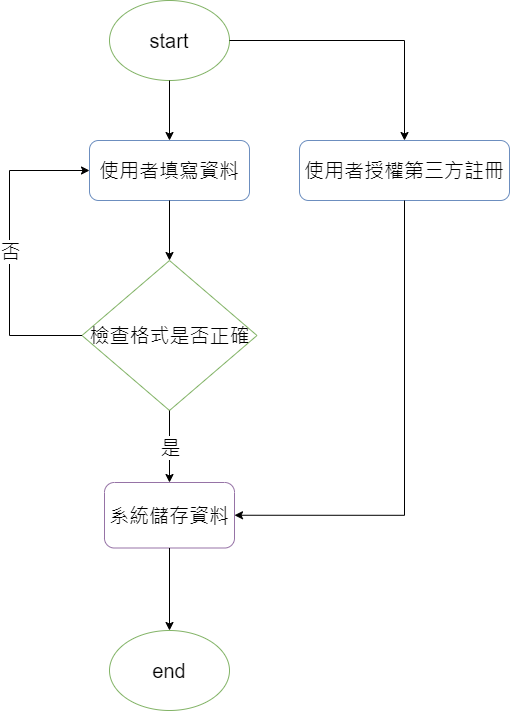
\includegraphics[width=0.5\textwidth]{assets/Process_Design/Register.png}
  \item 會員登入 \\
  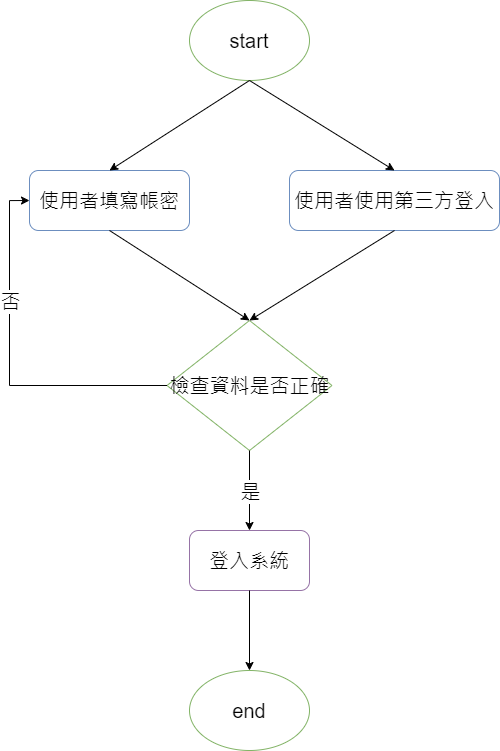
\includegraphics[width=0.5\textwidth]{assets/Process_Design/Login.png}
  \item 重設密碼 \\
  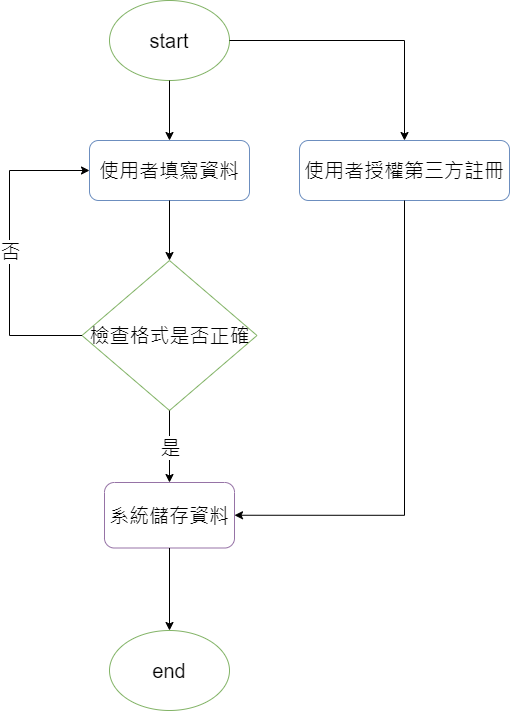
\includegraphics[width=0.5\textwidth]{assets/Process_Design/Register.png}
  \item 建立專案 \\
  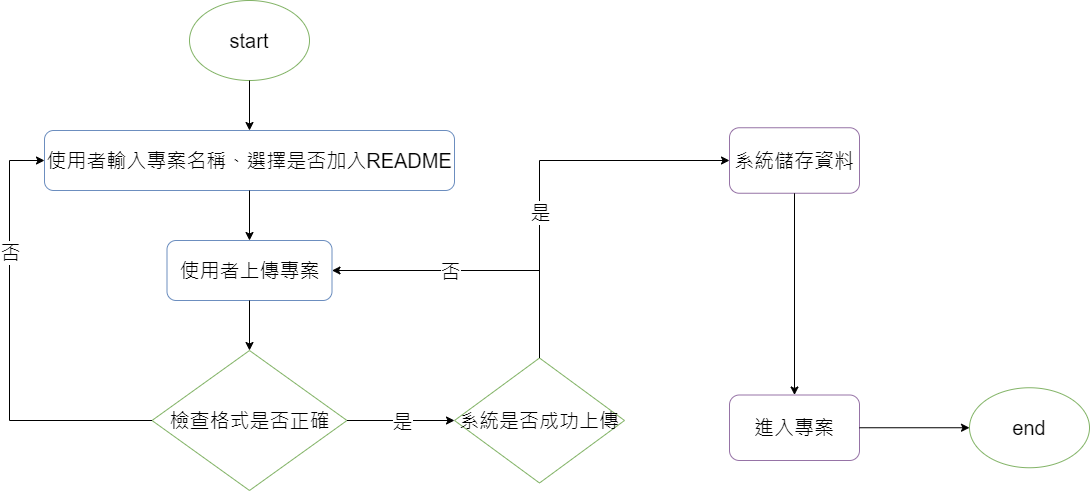
\includegraphics[width=0.8\textwidth]{assets/Process_Design/Create_Project.png}
  \item 編輯專案 \\
  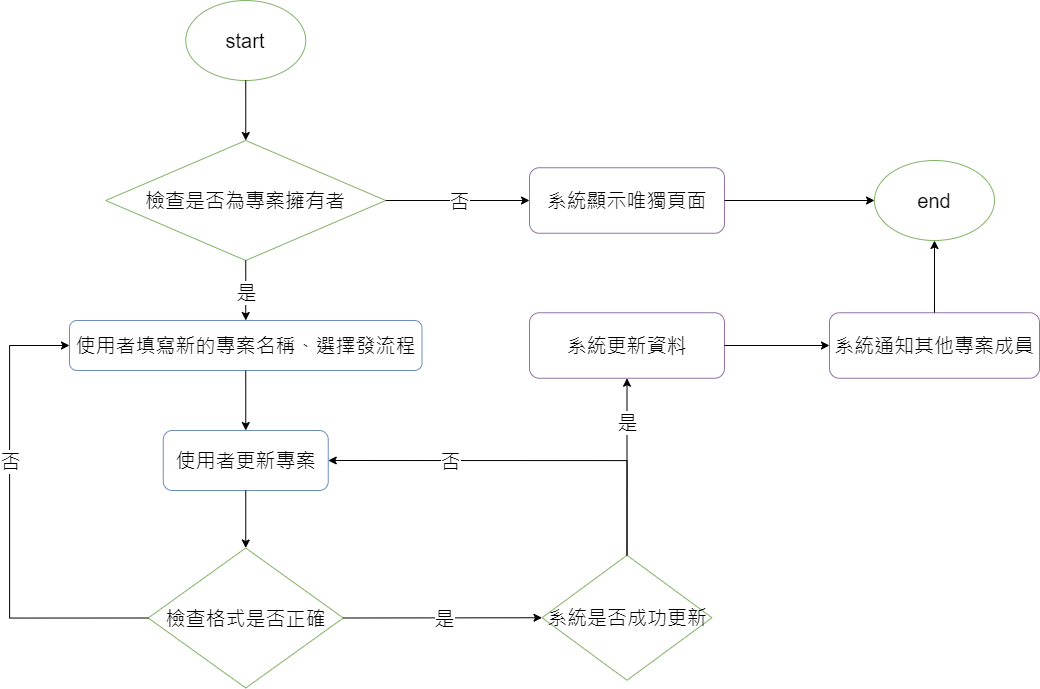
\includegraphics[width=0.8\textwidth]{assets/Process_Design/Edit_Project.png}
  \item 刪除專案 \\
  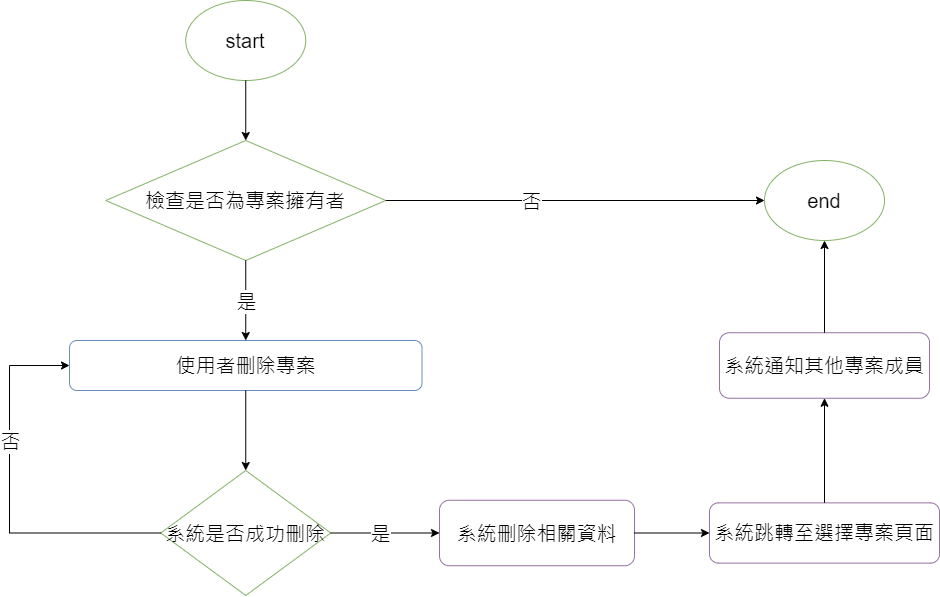
\includegraphics[width=0.8\textwidth]{assets/Process_Design/Delete_Project.png}
  \item 建立repository \\
  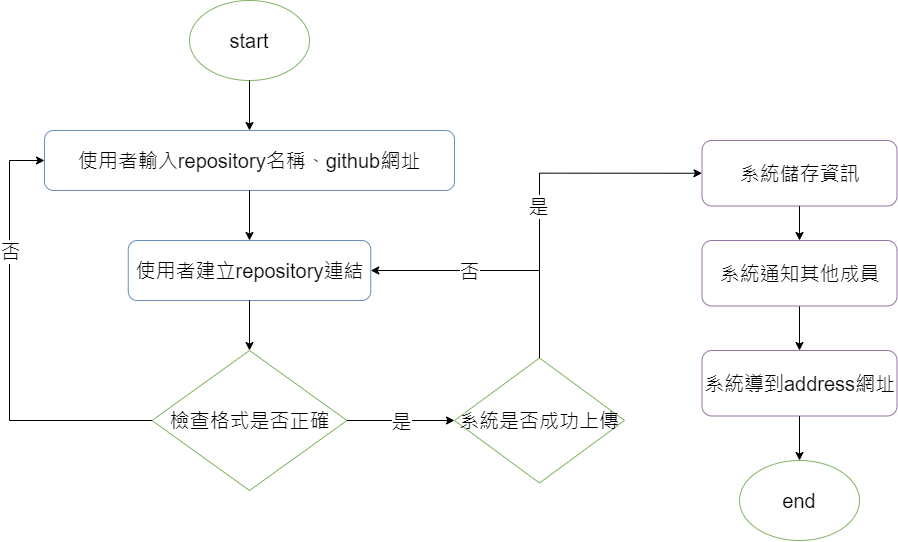
\includegraphics[width=0.8\textwidth]{assets/Process_Design/Create_repo.png}
  \item 刪除repository \\
  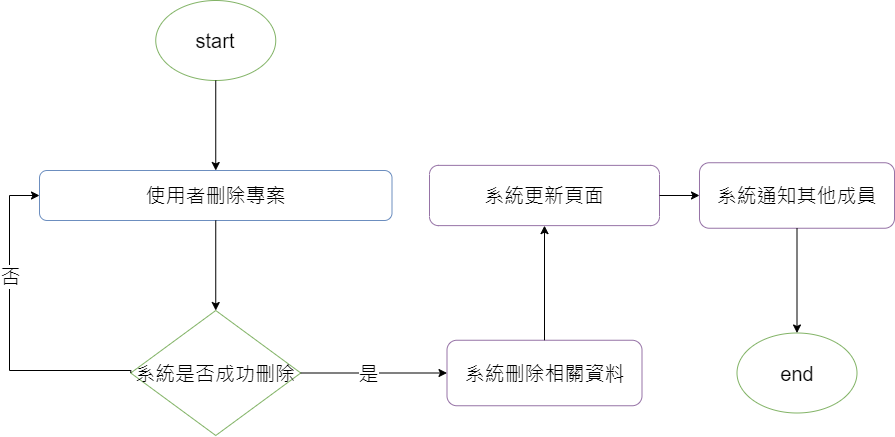
\includegraphics[width=0.8\textwidth]{assets/Process_Design/Delete_repo.png}
  \item 編輯文件 \\
  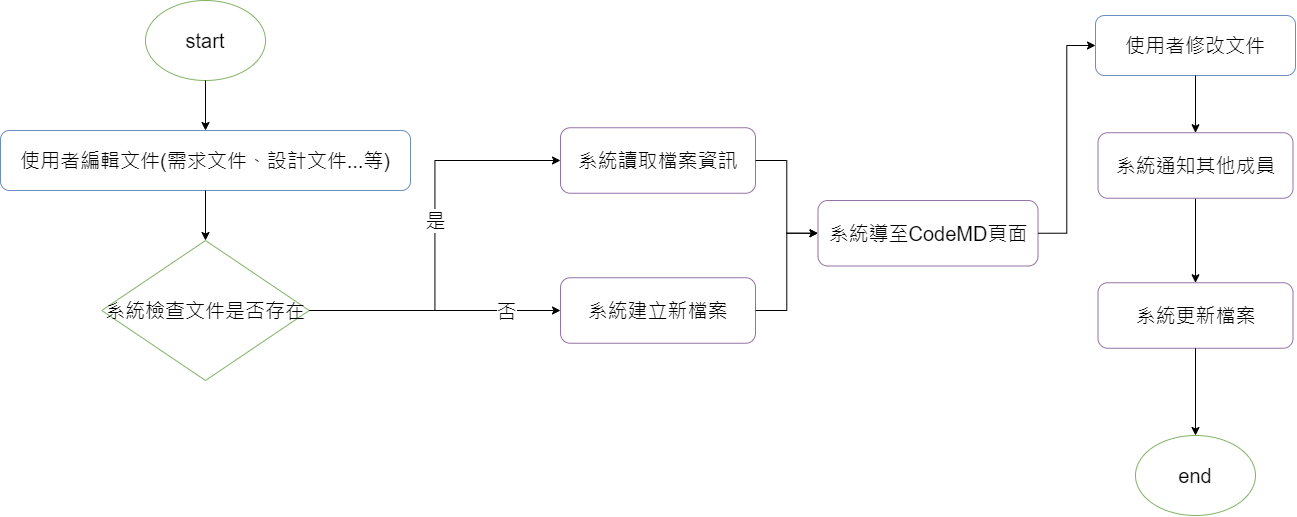
\includegraphics[width=0.8\textwidth]{assets/Process_Design/Edit_doc.png}
  \item 預覽文件 \\
  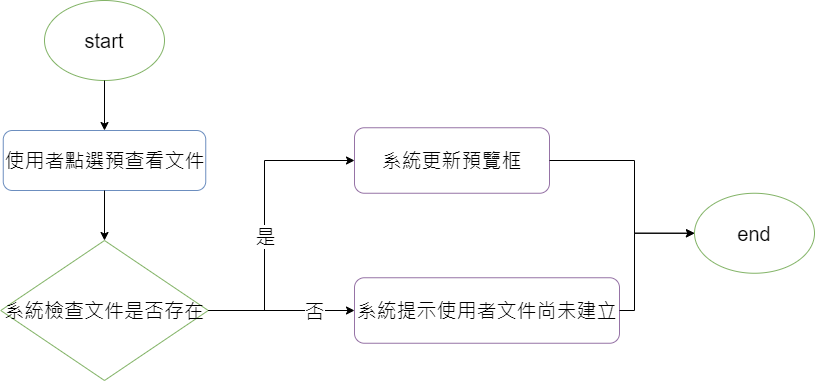
\includegraphics[width=0.8\textwidth]{assets/Process_Design/Preview_doc.png}
  \item 看板新增任務 \\
  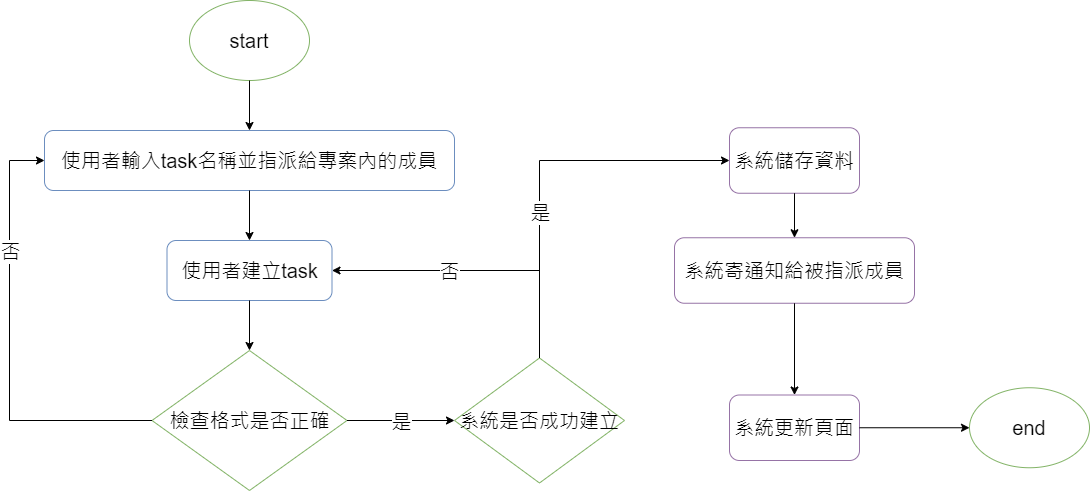
\includegraphics[width=0.8\textwidth]{assets/Process_Design/Create_task.png}
  \item 看板編輯任務 \\
  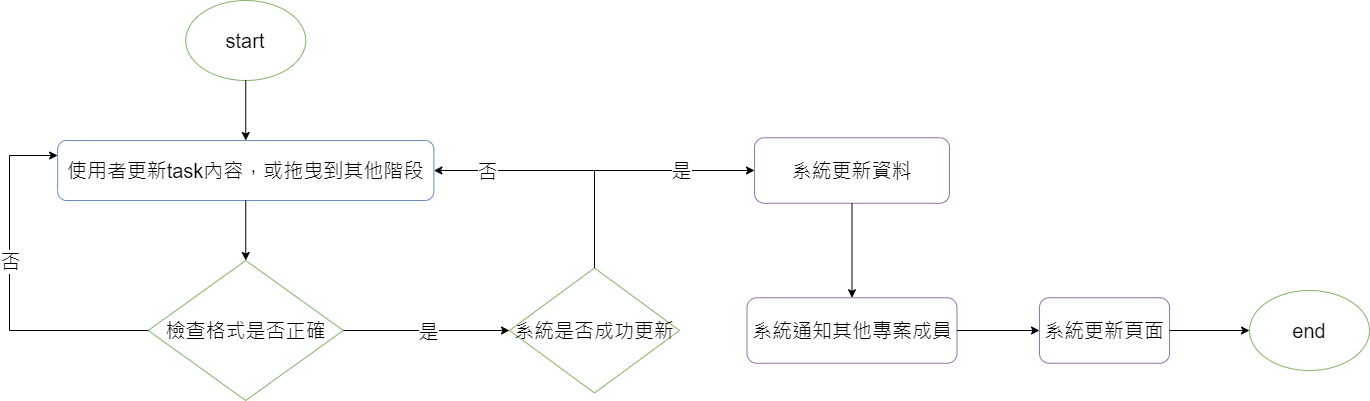
\includegraphics[width=0.8\textwidth]{assets/Process_Design/Edit_task.png}
  \item 看板刪除任務 \\
  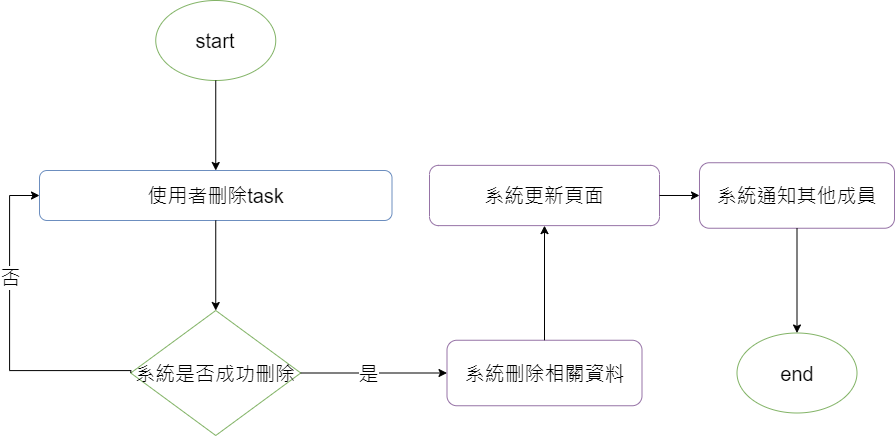
\includegraphics[width=0.5\textwidth]{assets/Process_Design/Delete_task.png}
  \item Q\&A文件\\
  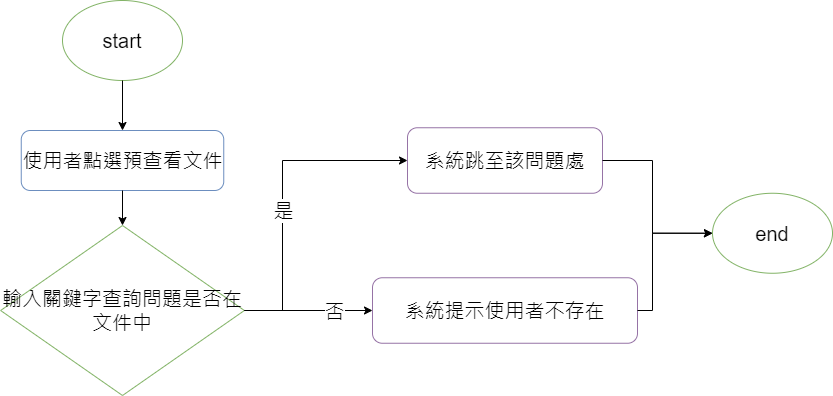
\includegraphics[width=0.8\textwidth]{assets/Process_Design/QA_doc.png}
  \item 變更成員 \\
  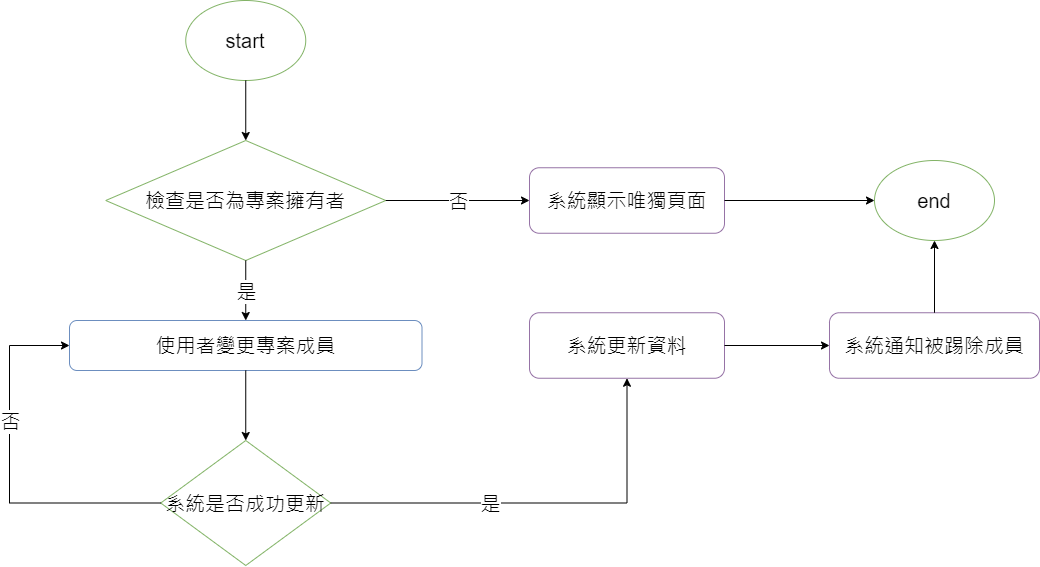
\includegraphics[width=0.8\textwidth]{assets/Process_Design/Change_Members.png}
  \item 邀請其他人 \\
  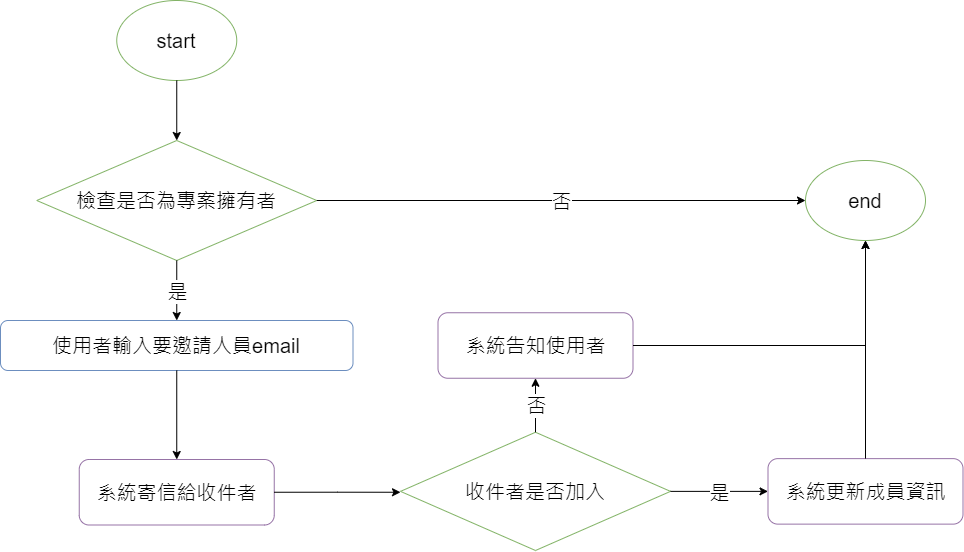
\includegraphics[width=0.8\textwidth]{assets/Process_Design/Join_Project.png}
  \item 邀請其他人 \\
  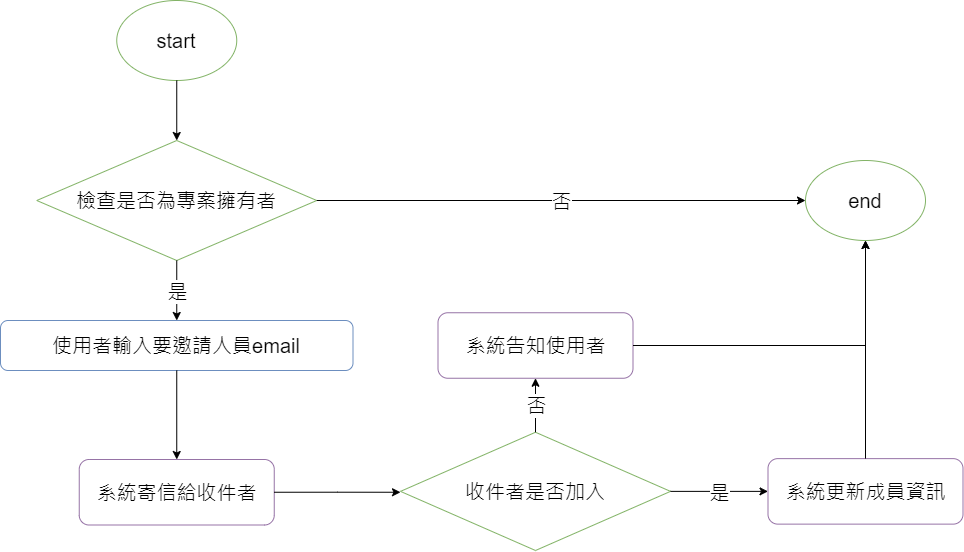
\includegraphics[width=0.8\textwidth]{assets/Process_Design/Join_Project.png}
  \item 設定個人資料 \\
  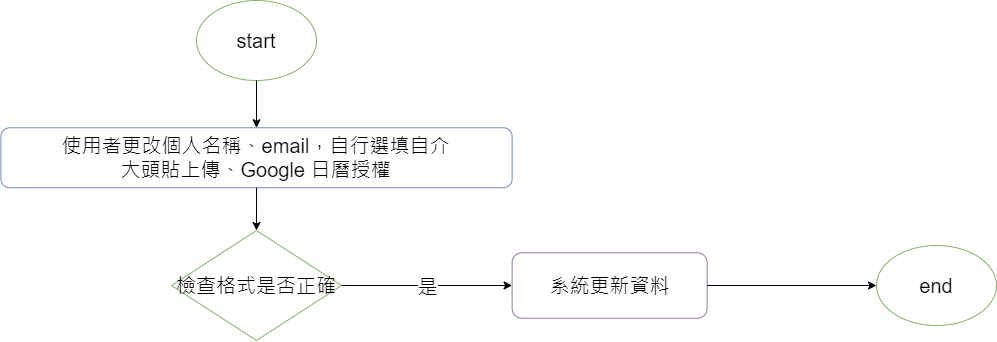
\includegraphics[width=0.8\textwidth]{assets/Process_Design/Set_Profile.png}
\end{enumerate}
\end{obeylines}

\section*{4. 使用者畫面設計(User Interface Design)}

\begin{obeylines}
\parindent=0pt
可用各種畫面設計方式,如發展網頁prototype、繪製PowerPoint投影片等,去設計你的主要系統畫面。此部份應是SRS中使用者介面分析的進階設計版本。
線框圖? 包含所有UI設計 版型顏色等等
CLI工具UI設計
何
\end{obeylines}

\section*{5. 資料設計(Data Design)}

\begin{obeylines}
\parindent=0pt
設計此系統的資料庫schema、檔案結構、XML schema、JSON (JavaScript Object Notation)物件等。
NoSQL 類似json格式
簡
\end{obeylines}

\section*{6. 類別圖設計(Class Diagram)}

\begin{obeylines}
\parindent=0pt
發展UML之class diagram (可對應C4 model中的Code diagram),明確設計系統中包含哪些類別,以及這些類別之間的關係。
若遇到非一般物件類別或特殊物件類別,如HTML、JavaScript、JSP、Servlet等,可用stereotype表達,如<<JavaScript>>、<<Servlet>>。
可把重點放在定義程式結構:訂出所有類別名稱、拉出所有類別關係,再加入重要的attibute/operation即可。而特殊的類別職責設計可加上文字說明。
	StarUML
	前後端都要
\end{obeylines}

\section*{7. 實作方案(Implementation Languages and Platforms)}

\begin{obeylines}
\parindent=0pt
說明系統之平台(如網站或行動App)
說明預計採用的程式語言或技術(如後端Java、node.js、PHP等,前端JS+Boostrap、Android、iOS等)
說明預計採用的框架(Framework,如前端React、Angular、Vue,後端Spring、SpringBoot等)、函式庫(如前端jQuery、d3.js,後端jsoup、iText)、Servless服務(Firebase)等。
輕輕鬆酥
\end{obeylines}

\section*{8. 設計議題(Design Issue)}

\begin{obeylines}
\parindent=0pt
將設計此系統過程中遭遇的議題紀錄下來,包含(1)議題內容、(2)可能解決方案(alternative solutions)、(3)最後解決方案(final solution)與理由(rationale)。
唐劭賢輕輕鬆酥
大家有問題都丟這邊ㄛ
\end{obeylines}

\end{document}
